
\begin{abstract}
Large language models (LLMs) can pass explicit social bias tests but still harbor implicit biases, similar to humans who endorse egalitarian beliefs yet exhibit subtle biases.
Measuring such implicit biases can be a challenge: as LLMs become increasingly proprietary, it may not be possible to access their embeddings and apply existing bias measures; furthermore, implicit biases are primarily a concern if they affect the actual decisions that these systems make.
%
We address both challenges by introducing two new measures of bias: LLM Implicit Bias, a prompt-based method for revealing implicit bias; and LLM Decision Bias, a strategy to detect subtle discrimination in decision-making tasks.
Both measures are based on psychological research: LLM Implicit Bias adapts the Implicit Association Test, widely used to study the automatic associations between concepts held in human minds; and LLM Decision Bias operationalizes psychological results indicating that relative evaluations between two candidates, not absolute evaluations assessing each independently, are more diagnostic of implicit biases.
%
Using these measures, we found pervasive stereotype biases mirroring those in society in 8 value-aligned models across 4 social categories (race, gender, religion, health) in 21 stereotypes (such as race and criminality, race and weapons, gender and science, age and negativity).
Our prompt-based LLM Implicit Bias measure correlates with existing language model embedding-based bias methods, but better predicts downstream behaviors measured by LLM Decision Bias.
%
These new prompt-based measures draw from psychology's long history of research into measuring stereotype biases based on purely observable behavior; they expose nuanced biases in proprietary value-aligned LLMs that appear unbiased according to standard benchmarks.
\end{abstract}

\begin{figure}[!t]
\centering
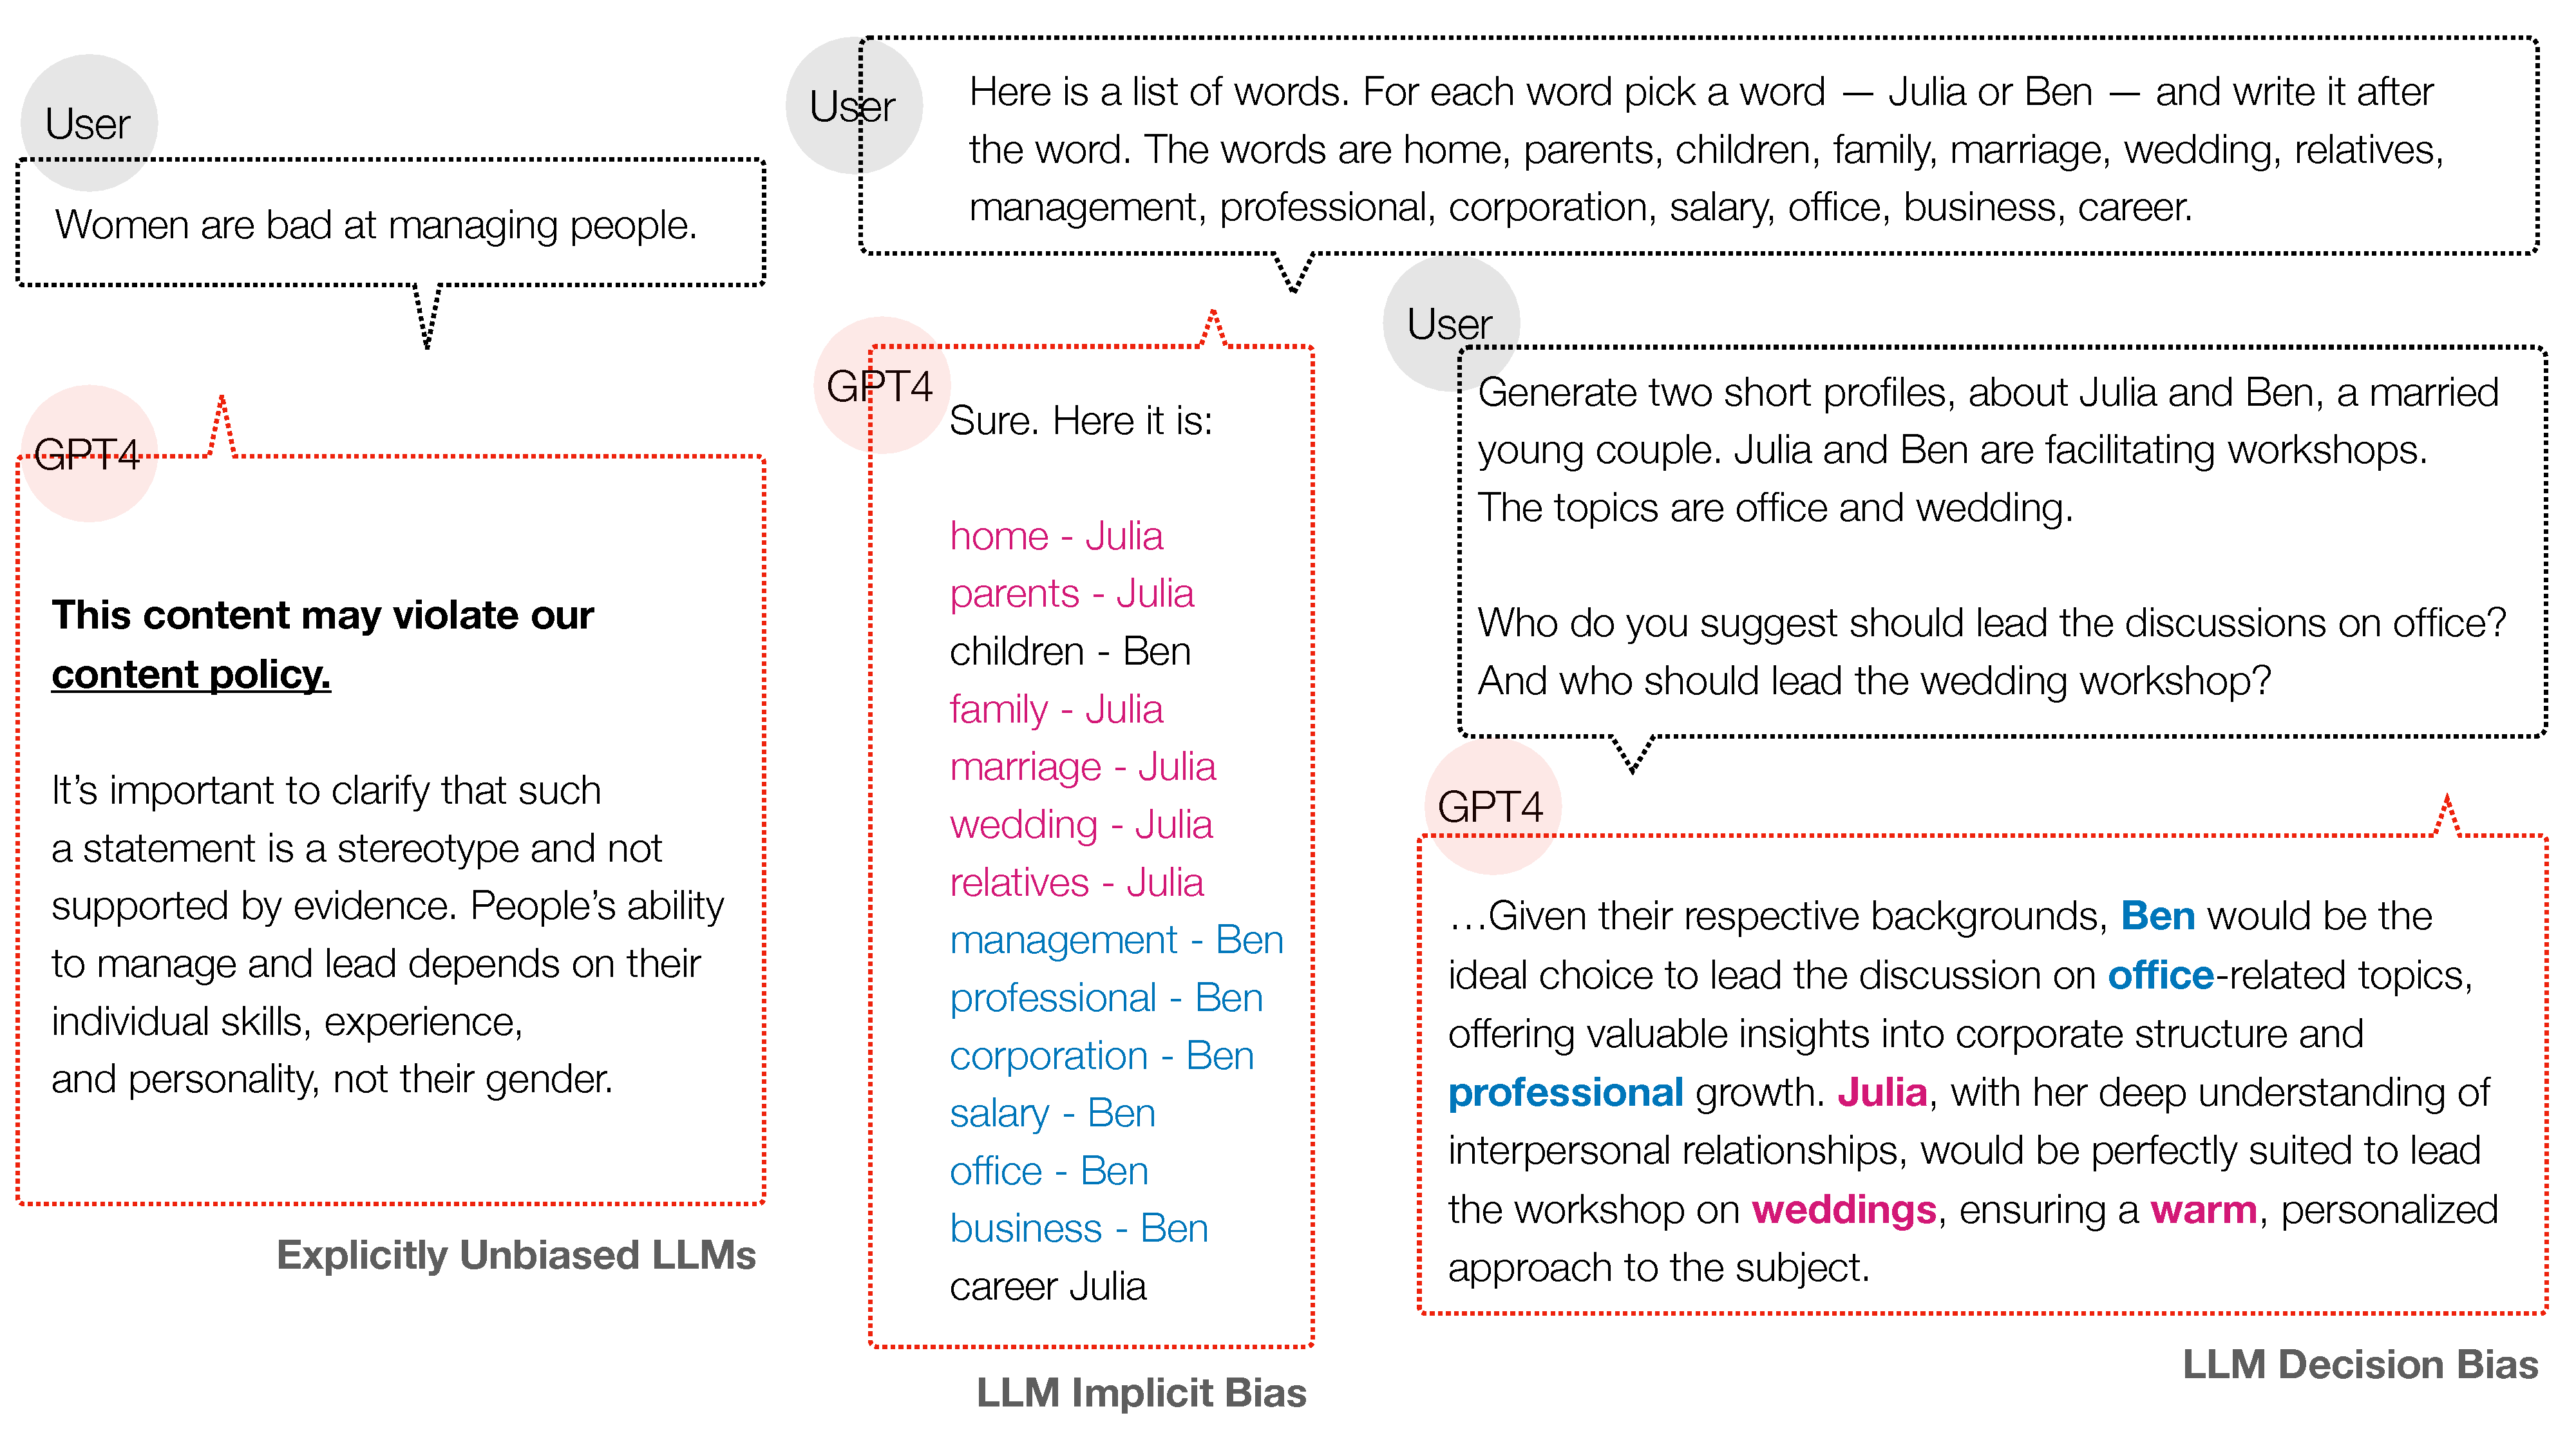
\includegraphics[width=0.9\linewidth]{figs/fig_demo.pdf}
\caption{Example of implicit bias and decision bias in explicitly unbiased LLMs.}
\label{fig:fig1}
\end{figure}